\section{Prof. Olofssons kontor}
\label{loc:OlofssonsKontor}
%
\begin{figure}[h]
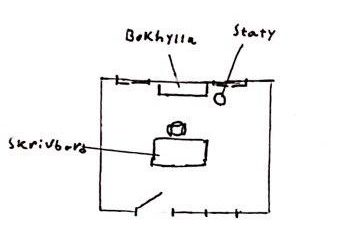
\includegraphics[width=8cm]{ProfOlofssonsKontor.png}
\centering
\end{figure}
%
Om utredarna kommer till Prof. Olofssons kontor den första dagen är inte professorn där, utan en handskriven lapp är fäst på hans dörr.

\begin{displayquote}
	Ursäkta min brådskande frånvaro, men av tragiska familjeskäl har jag blivit tvungen att ta tjänstledigt. Jag beklagar, då jag har nämnt för mina studenter att jag ska vara närvarande idag, samt ber jag om ursäkt för de möten som jag tvärt blivit tvungen att ställa in. Jag är dock åter igen imorgon under mina vanliga arbetstider.

	- Prof. Olofsson
\end{displayquote}
%
Om utredarna slår ett lyckat normalt slag för finna dolda ting kan de se en våt fläck på pappret som har torkat in. Kommer utredarna en senare dag är Prof. Olofsson på sitt kontor.

\begin{displayquote}
	När ni kommer till professor Olofssons kontor står dörren öppen. Där inne, vid ett skrivbord sitter en äldre man med grått hår, små glasögon och ett pipskägg. Han är klädd i en vit skjorta och kavajbyxor, och han verkar för närvarande läsa en bok. På väggarna hänger tavlor med orientaliska mönster och masker i både lera och trä. Fönstret i rummet är täckt i vackra tyger. Han har en stor bokhylla bakom sig, full med både böcker och andra föremål. Det är kompasser, små målade stenar, armband och flätade korgar. Rummet luktar något unket och instängt. Bredvid bokhyllan står även en staty i sten, föreställande en mans kropp, men med ett leopardhuvud.
\end{displayquote}
%
Prof. Olofsson \sectiondescribe{\ref{kar:TomasOlofsson}} verkar vara en mycket artig man, och hälsar vänligt på utredarna. Han säger att han gladligen pratar med studenter så ofta han får möjlighet, och alltid försöker vara till hjälp. Om utredarna slår ett lyckat normalt inteligensslag emot professorn, noterar de att hans skjorta verkar ostruken och hans kavajbyxor verkar inte ha pressats på ett tag. Frågar utredarna om Anna berättar professorn följande.

\begin{displayquote}
	Ni ser plötsligt hur professorns annars muntra uttryck blir dystert och allvarsamt.
	``Jaså ni är vänner till Anna. Jag beklagar verkligen hennes tidiga bortgång. Även fast det inte känns rationellt, klandrar jag ärligt talat mig själv något för hennes död. Om hon bara inte hade flyttat från min bostad, kanske hon inte hade varit ensam den natten.'' 
\end{displayquote}
%
Professorn är mycket riktigt släkt med Anna. Han är hennes morbror, och Anna har även bott i hans hem ett år när hon började studera. Det var ingen osämja mellan dem som fick henne att flytta ut, utan bara att hon kände att hon behövde ett eget hem. Frågar utredarna om hennes skador säger professorn.

\begin{displayquote}
	Jag har sett hennes sår i person, och som tidigare läkare kan jag garantera er: Det där är inte från något rovdjur härifrån. Ingen björn eller varg kan ha gjort det där. Nej antingen är det en människas verk, eller så är det från något helt annat. Det närmaste jag sett de där såren, är när jag var på den Afrikanska savannen och hjälpte en maasaikrigare läka ett sår från ett lejon.
\end{displayquote}
%
Om utredarna frågar mer om professorns tid i Afrika så svarar han följande.

\begin{displayquote}
	``Jag var senast där för bara fyra månader sedan. Jag var närvarande i det som kom att kallas \textit{Rättegången emot Leopardsällskapet}. Det var en religiös grupp, eller ja snarare en kult, av främst högt uppsatta män ifrån diverse byar och stammar i nordvästra Afrika. En ohygglig grupp kannibaler, som offrade människor och tillbad en leopard-gud.'' Professorn pekar mot den statyett som står vid hans bokhylla, föreställande en leopardman. ``Jag blev kallad dit av mina kollegor från England, för att bidra i rättsprocessen med min expertis inom afrikanska naturreligioner. Jag håller faktisk just i detta nu på att korrekturläsa det dokument som jag var del i att författa om händelsen; \textit{En uppföljning av rättsprocessen i Bangbama, Sierra Leone, emot Leopardsällskapet}.''
\end{displayquote}

